\begin{experiment}{Approaches to deal with the curse of dimensionality.}{\small \sffamily\textbf{Description}

We are testing limit on range 1---35 using heart dataset, analyzing:

\begin{itemize}
\tightlist
	\item \texttt{RAN} --- \emph{Random \emph{exposers}}, an ensemble, using \textbf{random} approach, grain \emph{30}, radius \emph{0.1}, dimensions \emph{[2]}, using \textbf{single measure per class}.
	\item \texttt{HEU} --- \emph{Heuristic approach}, an ensemble, using \textbf{heuristic} approach, grain \emph{30}, radius \emph{0.1}, pool \emph{78}, dimensions \emph{[2]}, using \textbf{single measure per class}.

\end{itemize}


\textbf{Results}

\centering
	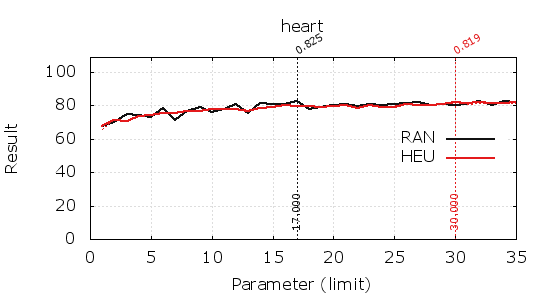
\includegraphics[width=.75\textwidth]{plots/experiment_8_heart.png}
	\captionof{figure}{Approaches to deal with the curse of dimensionality.}
	\label{fig:experiment_8}
}\end{experiment}